%%%%%%%%%%%%%%%%%%%%%%%%%%%%%%%%%%%%%%%%%%%%%%%%%%%%%%%
% INTRODUCCION A LAS GEODESICAS EN ESPACIOS METRICOS
%%%%%%%%%%%%%%%%%%%%%%%%%%%%%%%%%%%%%%%%%%%%%%%%%%%%%%%
\RequirePackage{fix-cm}
\documentclass[12pt, a4paper]{amsart}

\usepackage[utf8]{inputenc}
\usepackage{amssymb}
\usepackage{mathtools}
\usepackage{enumitem}
\usepackage{array}
\usepackage{tikz}
\usepackage{fancyhdr}
\usepackage{hyperref}

\hfuzz2pt

%% Colores del Instituto de Cálculo y del Departamento de Matemática
\definecolor{icnavy}{HTML}{013274}
\definecolor{iccyan}{HTML}{029BDF}
\definecolor{icmag}{HTML}{E2017B}
\definecolor{dmred}{HTML}{A8000C}
\hypersetup{colorlinks=true,linkcolor=icnavy,citecolor=icnavy,urlcolor=icnavy,
  pdftitle={Introducción a las geodésicas en espacios métricos},
  pdfauthor={Julián Fernández Bonder}}

\setlength{\textwidth}{15.5cm}
\setlength{\textheight}{23cm}
\setlength{\oddsidemargin}{0.2cm}
\setlength{\evensidemargin}{0.2cm}
\calclayout
\parskip 3pt

%% Encabezados
\pagestyle{fancy}
\fancyhf{}
\fancyhead[C]{\footnotesize\scshape\color{icnavy}Introducción a las geodésicas en espacios métricos}
\fancyhead[R]{\footnotesize\thepage}
\renewcommand{\headrulewidth}{0pt}

%% Teoremas
\newtheorem{teorema}{Teorema}[section]
\newtheorem{proposicion}[teorema]{Proposición}
\newtheorem{lema}[teorema]{Lema}
\newtheorem{corolario}[teorema]{Corolario}
\theoremstyle{definition}
\newtheorem{definicion}[teorema]{Definición}
\newtheorem{ejemplo}[teorema]{Ejemplo}
\theoremstyle{remark}
\newtheorem{observacion}[teorema]{Observación}

\renewcommand{\proofname}{Demostración}
\renewcommand{\figurename}{Figura}

\newcommand{\Bc}{\overline{B}}
\newcommand{\ve}{\varepsilon}

\begin{document}

%%
%% TÍTULO
%%
\thispagestyle{plain}
\begin{flushleft}
  {\color{icnavy}\fontsize{26}{29}\selectfont\bfseries
   Introducción a las geodésicas\\ en espacios métricos\par}
  \vspace{10pt}
  {\color{dmred}\rule{\textwidth}{1.2pt}}\par
  \vspace{6pt}
  {\color{icnavy!75}\large Julián Fernández Bonder\par}
  \vspace{3pt}
  {\color{icnavy!60}\small Instituto de Cálculo, FCEN--CONICET \quad$\cdot$\quad Departamento de Matemática, FCEN--UBA\par}
\end{flushleft}
\vspace{1.2cm}


\section{Longitud de curvas}

Sea $(X,d)$ un espacio métrico y sea $\gamma\colon[a,b]\to X$ una curva continua. La \emph{longitud} de $\gamma$ se define por
\[
L(\gamma) := \sup\left\{\sum_{i=1}^n d\big(\gamma(t_i),\gamma(t_{i-1})\big) : a=t_0<t_1<\dots<t_n=b\right\}\in[0,\infty].
\]
Cuando haya más de una métrica en juego escribiremos $L_d(\gamma)$.

\begin{definicion}
La curva $\gamma$ es \emph{rectificable} si $L(\gamma)<\infty$.
\end{definicion}

Cada suma de la definición es la longitud de la ``poligonal'' que une los puntos $\gamma(t_0),\gamma(t_1),\dots,\gamma(t_n)$, en la que cada tramo se mide con la distancia $d$ (Figura~\ref{fig:poligonal}). Por la desigualdad triangular, agregar puntos a la partición no disminuye la suma, así que la longitud es el límite de estas sumas a medida que la partición se refina.

\begin{figure}[htbp]
\centering
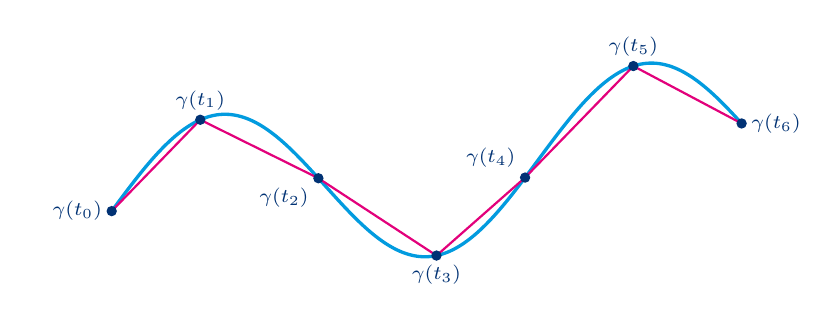
\begin{tikzpicture}[scale=1.25, declare function={f(\x)=1+0.85*sin(deg(1.45*\x))+0.12*\x;}]
  \draw[iccyan, very thick] plot[domain=0:6.4, samples=200, smooth] (\x,{f(\x)});
  \draw[icmag, thick] plot[samples at={0,0.9,2.1,3.3,4.2,5.3,6.4}] (\x,{f(\x)});
  \foreach \t/\lab/\pos in {0/0/left, 0.9/1/above, 2.1/2/below left, 3.3/3/below, 4.2/4/above left, 5.3/5/above, 6.4/6/right}
    \fill[icnavy] (\t,{f(\t)}) circle (1.5pt) node[\pos] {\scriptsize $\gamma(t_{\lab})$};
\end{tikzpicture}
\caption{La curva $\gamma$ (en cian) y la poligonal inscripta asociada a una partición $t_0<\dots<t_6$ (en magenta). La longitud de la poligonal es $\sum_i d(\gamma(t_{i-1}),\gamma(t_i))\le L(\gamma)$.}
\label{fig:poligonal}
\end{figure}

Por la desigualdad triangular, toda curva que une $x$ con $y$ satisface $d(x,y)\le L(\gamma)$. Más en general, si $s\le t$, entonces $d(\gamma(s),\gamma(t))\le L(\gamma|_{[s,t]})$.

\begin{ejemplo}[Arcos de circunferencia]\label{ej:arco}
Sea $S^1=\{z\in\mathbb R^2:|z|=1\}$ con la distancia euclídea $d(z,w)=|z-w|$, y sea $\gamma(t)=(\cos t,\sin t)$ para $t\in[0,\theta]$, con $0<\theta\le2\pi$. Veamos que $L(\gamma)=\theta$, es decir, que la definición de longitud da la longitud de arco usual.

Para $s\le t$, la cuerda entre $\gamma(s)$ y $\gamma(t)$ mide
\[
|\gamma(t)-\gamma(s)|=2\sin\Big(\frac{t-s}{2}\Big)\le t-s,
\]
porque $\sin u\le u$ para $u\ge0$. Sumando sobre cualquier partición de $[0,\theta]$, cada suma es a lo sumo $\theta$, y entonces $L(\gamma)\le\theta$. Por otro lado, para la partición en $n$ partes iguales todas las cuerdas miden lo mismo (Figura~\ref{fig:arco}), y
\[
\sum_{i=1}^n d\big(\gamma(t_{i-1}),\gamma(t_i)\big)=2n\sin\Big(\frac{\theta}{2n}\Big)\xrightarrow[n\to\infty]{}\theta,
\]
porque $\sin u/u\to1$ cuando $u\to0$. Luego $L(\gamma)=\theta$.
\end{ejemplo}

\begin{figure}[htbp]
\centering
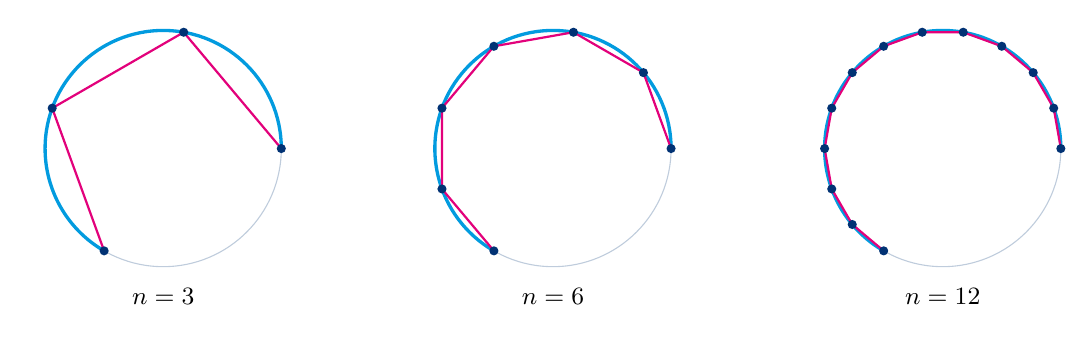
\begin{tikzpicture}[scale=1.5]
  \foreach \n/\xs in {3/0, 6/3.3, 12/6.6}{
    \begin{scope}[xshift=\xs cm]
      \draw[icnavy!25] (0,0) circle (1);
      \draw[iccyan, very thick] (0:1) arc (0:240:1);
      \draw[icmag, thick] plot[domain=0:\n, samples=\n+1] ({cos(240*\x/\n)},{sin(240*\x/\n)});
      \foreach \k in {0,...,\n} \fill[icnavy] ({cos(240*\k/\n)},{sin(240*\k/\n)}) circle (1.1pt);
      \node[below] at (0,-1.1) {\small $n=\n$};
    \end{scope}}
\end{tikzpicture}
\caption{Poligonales inscriptas en un arco de ángulo $\theta=\frac{4\pi}{3}$ con particiones uniformes de $n$ partes. Sus longitudes, $2n\sin(\theta/2n)$, crecen hacia $\theta$.}
\label{fig:arco}
\end{figure}

\begin{lema}[Aditividad]\label{lem:aditividad}
Si $a\le c\le b$, entonces $L(\gamma)=L(\gamma|_{[a,c]})+L(\gamma|_{[c,b]})$.
\end{lema}

\begin{proof}
Si $P$ es una partición de $[a,b]$, agregarle el punto $c$ no disminuye la suma correspondiente (desigualdad triangular), y la partición resultante se separa en una de $[a,c]$ y una de $[c,b]$. Luego la suma de $P$ es a lo sumo $L(\gamma|_{[a,c]})+L(\gamma|_{[c,b]})$, y tomando supremo sale ``$\le$''. Recíprocamente, juntando una partición de $[a,c]$ con una de $[c,b]$ se obtiene una de $[a,b]$, cuya suma es la suma de ambas; tomando supremos por separado sale ``$\ge$''.
\end{proof}

\begin{lema}[Continuidad de la longitud acumulada]\label{lem:continuidad}
Sea $\gamma\colon[a,b]\to X$ rectificable y $\ell(t):=L(\gamma|_{[a,t]})$. Entonces $\ell$ es continua y no decreciente, con $\ell(a)=0$ y $\ell(b)=L(\gamma)$.
\end{lema}

\begin{proof}
La monotonía es consecuencia del Lema~\ref{lem:aditividad}, que además da $\ell(t)-\ell(s)=L(\gamma|_{[s,t]})$ para $s\le t$. Veamos la continuidad por derecha en $t_0\in[a,b)$; la continuidad por izquierda es análoga.

Sea $\varepsilon>0$. Elegimos una partición $t_0<t_1<\dots<t_n=b$ de $[t_0,b]$ con
\[
\sum_{i=1}^n d(\gamma(t_{i-1}),\gamma(t_i)) > L(\gamma|_{[t_0,b]})-\varepsilon.
\]
Por continuidad de $\gamma$, existe $t\in(t_0,t_1)$ con $d(\gamma(t_0),\gamma(t))<\varepsilon$. Agregando $t$ a la partición la suma no disminuye, de modo que
\[
L(\gamma|_{[t_0,b]})-\varepsilon < d(\gamma(t_0),\gamma(t)) + d(\gamma(t),\gamma(t_1)) + \sum_{i=2}^n d(\gamma(t_{i-1}),\gamma(t_i)) \le \varepsilon + L(\gamma|_{[t,b]}).
\]
Como todas las longitudes son finitas, por aditividad $\ell(t)-\ell(t_0)=L(\gamma|_{[t_0,b]})-L(\gamma|_{[t,b]})<2\varepsilon$. Por monotonía lo mismo vale para todo $t'\in(t_0,t]$, lo que prueba la continuidad por derecha.
\end{proof}

\begin{lema}[Semicontinuidad inferior]\label{lem:sci}
Sean $\gamma_n,\gamma\colon[a,b]\to X$ curvas tales que $\gamma_n(t)\to\gamma(t)$ para todo $t\in[a,b]$. Entonces
\[
L(\gamma)\le\liminf_{n\to\infty}L(\gamma_n).
\]
\end{lema}

\begin{proof}
Para una partición $a=t_0<\dots<t_k=b$ fija, por continuidad de $d$,
\[
\sum_{i=1}^k d(\gamma(t_{i-1}),\gamma(t_i)) = \lim_{n\to\infty}\sum_{i=1}^k d(\gamma_n(t_{i-1}),\gamma_n(t_i)) \le \liminf_{n\to\infty} L(\gamma_n).
\]
Tomando supremo sobre las particiones se obtiene el resultado.
\end{proof}

\begin{observacion}
En el Lema~\ref{lem:sci} alcanza con convergencia \emph{puntual}; en particular vale para convergencia uniforme, que es la que aparece en la demostración del Teorema~\ref{thm:HR}.
\end{observacion}

\section{Espacios de longitud}

\begin{definicion}
El espacio métrico $(X,d)$ es un \emph{espacio de longitud} si, para todo $x,y\in X$ y todo $\varepsilon>0$, existe una curva rectificable $\gamma\colon[0,1]\to X$ con $\gamma(0)=x$, $\gamma(1)=y$ y
\[
L(\gamma)<d(x,y)+\varepsilon.
\]
Equivalentemente, la distancia entre dos puntos es el ínfimo de las longitudes de las curvas que los unen.
\end{definicion}

\subsection{La métrica intrínseca}

Supongamos ahora que $(X,d)$ es un espacio métrico cualquiera en el que todo par de puntos se puede unir con una curva rectificable. Definimos
\[
d_L(x,y):=\inf\{L_d(\gamma) : \gamma \text{ es una curva que une } x \text{ con } y\}.
\]

\begin{proposicion}\label{prop:dL-metrica}
$d_L$ es una métrica en $X$ y $d\le d_L$.
\end{proposicion}

\begin{proof}
La finitud de $d_L$ es exactamente la hipótesis de que todo par de puntos se une con una curva rectificable; sin ella, $d_L$ sería una métrica extendida (con valores en $[0,\infty]$). Como $d(x,y)\le L_d(\gamma)$ para toda curva que une $x$ con $y$, tomando ínfimo se obtiene $d\le d_L$; en particular, $d_L(x,y)=0$ implica $x=y$. La simetría sale de que la curva recorrida al revés tiene la misma longitud. Para la desigualdad triangular, si $\gamma_1$ une $x$ con $y$ y $\gamma_2$ une $y$ con $z$, su concatenación une $x$ con $z$ y, por el Lema~\ref{lem:aditividad}, tiene longitud $L_d(\gamma_1)+L_d(\gamma_2)$. Tomando ínfimos, $d_L(x,z)\le d_L(x,y)+d_L(y,z)$.
\end{proof}

\begin{observacion}
Como $d\le d_L$, la topología de $d_L$ es más fina o igual que la de $d$, y en general puede ser estrictamente más fina.
\end{observacion}

\begin{ejemplo}[La circunferencia y la esfera]\label{ej:esfera}
Volvamos a $S^1\subset\mathbb R^2$ con la distancia euclídea $d(z,w)=|z-w|$. Dados $z,w\in S^1$, sea $\theta\in[0,\pi]$ el ángulo entre ellos, es decir, $\cos\theta=\langle z,w\rangle$. Entonces:

\begin{itemize}
\item La distancia euclídea es la longitud de la cuerda: $d(z,w)=2\sin(\theta/2)$.
\item La distancia intrínseca es la longitud del arco más corto: $d_L(z,w)=\theta$.
\end{itemize}

Para la segunda afirmación, el arco más corto tiene longitud $\theta$ por el Ejemplo~\ref{ej:arco}, así que $d_L(z,w)\le\theta$. Recíprocamente, toda curva $\gamma$ en $S^1$ de $z$ a $w$ se puede escribir como $\gamma(t)=(\cos\varphi(t),\sin\varphi(t))$ con $\varphi$ continua (el argumento continuo), y $|\varphi(1)-\varphi(0)|\ge\theta$. Tomando particiones finas, donde las cuerdas $2\sin(|\Delta\varphi_i|/2)$ son casi iguales a los incrementos $|\Delta\varphi_i|$, se obtiene $L(\gamma)\ge\sum_i|\Delta\varphi_i|\ge\theta$, salvo un error arbitrariamente chico. Luego $d_L(z,w)=\theta$.

Como $2\sin(\theta/2)<\theta$ para $\theta>0$, el espacio $(S^1,d)$ \emph{no} es de longitud: la cuerda que realiza la distancia euclídea se sale de la circunferencia, y toda curva dentro de $S^1$ es más larga (Figura~\ref{fig:esfera}, izquierda).

Sin embargo, las dos métricas son \emph{equivalentes}. Como $\sin$ es cóncava en $[0,\pi/2]$, vale $\sin u\ge\frac{2}{\pi}u$ para $u\in[0,\frac\pi2]$; con $u=\theta/2$ se obtiene $\theta\le\frac\pi2\cdot2\sin(\theta/2)$. Es decir,
\[
d(z,w)\le d_L(z,w)\le\frac{\pi}{2}\,d(z,w)\qquad(z,w\in S^1).
\]
La constante $\frac\pi2$ es óptima: se alcanza en puntos antipodales, donde $d=2$ y $d_L=\pi$. En particular, $d$ y $d_L$ tienen las mismas sucesiones convergentes y las mismas sucesiones de Cauchy.

Lo mismo ocurre en la esfera $S^2\subset\mathbb R^3$ (Figura~\ref{fig:esfera}, derecha). Si $\theta\in[0,\pi]$ es el ángulo entre $z$ y $w$, la distancia euclídea es otra vez $2\sin(\theta/2)$, y la distancia intrínseca es $\theta$: es la longitud del arco más corto del \emph{círculo máximo} que pasa por $z$ y $w$ (la intersección de $S^2$ con el plano que contiene a $0$, $z$ y $w$). Que ningún otro camino sobre la esfera sea más corto es un hecho clásico que aceptamos sin demostración. La desigualdad $d\le d_L\le\frac\pi2 d$ vale con la misma cuenta.
\end{ejemplo}

\begin{figure}[htbp]
\centering
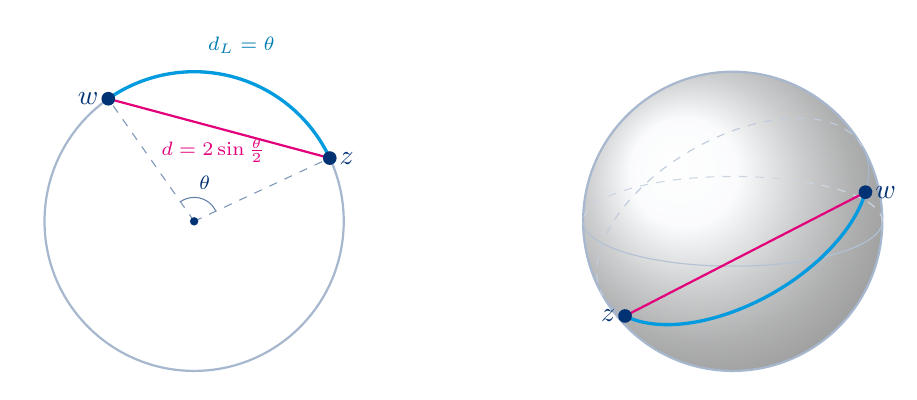
\begin{tikzpicture}[scale=1.9]
  % circunferencia
  \draw[icnavy!35, thick] (0,0) circle (1);
  \coordinate (O) at (0,0);
  \coordinate (Z) at (25:1);
  \coordinate (W) at (125:1);
  \draw[iccyan, very thick] (25:1) arc (25:125:1);
  \draw[icmag, thick] (Z) -- (W);
  \draw[icnavy!50, dashed] (O) -- (Z) (O) -- (W);
  \draw[icnavy!60] (25:0.16) arc (25:125:0.16);
  \node[icnavy] at (75:0.27) {\scriptsize $\theta$};
  \fill[icnavy] (Z) circle (1.3pt) node[right] {$z$};
  \fill[icnavy] (W) circle (1.3pt) node[left] {$w$};
  \fill[icnavy] (O) circle (0.8pt);
  \node[iccyan!80!black] at (75:1.22) {\scriptsize $d_L=\theta$};
  \node[icmag] at (75:0.49) {\scriptsize $d=2\sin\frac\theta2$};
  % esfera
  \begin{scope}[xshift=3.6cm]
    \shade[ball color=icnavy!4, opacity=0.6] (0,0) circle (1);
    \draw[icnavy!35, thick] (0,0) circle (1);
    \draw[icnavy!30] (-1,0) arc (180:360:1 and 0.3);
    \draw[icnavy!20, dashed] (1,0) arc (0:180:1 and 0.3);
    \begin{scope}[rotate=30]
      \draw[icnavy!25, dashed] (0:1 and 0.55) arc (0:180:1 and 0.55);
      \draw[icnavy!35] (180:1 and 0.55) arc (180:360:1 and 0.55);
      \draw[iccyan, very thick] (200:1 and 0.55) arc (200:330:1 and 0.55);
      \draw[icmag, thick] (200:1 and 0.55) -- (330:1 and 0.55);
      \fill[icnavy] (200:1 and 0.55) circle (1.3pt) node[left] {$z$};
      \fill[icnavy] (330:1 and 0.55) circle (1.3pt) node[right] {$w$};
    \end{scope}
  \end{scope}
\end{tikzpicture}
\caption{Izquierda: en $S^1$, la distancia euclídea es la longitud de la cuerda (magenta) y la distancia intrínseca es la del arco más corto (cian). Derecha: en $S^2$, el arco más corto es un arco de círculo máximo.}
\label{fig:esfera}
\end{figure}

El ejemplo siguiente muestra que, en cambio, $d$ y $d_L$ pueden no ser equivalentes, e incluso definir topologías distintas.

\begin{ejemplo}[El peine]\label{ej:peine}
Sea $X\subset\mathbb{R}^2$ la unión de $[0,1]\times\{0\}$, de $\{0\}\times[0,1]$ y de los segmentos $\{1/n\}\times[0,1]$, $n\ge1$, con la métrica euclídea $d$. Sean $p_n=(1/n,1)$ y $p=(0,1)$. Entonces $d(p_n,p)=1/n\to0$, pero toda curva en $X$ que une $p_n$ con $p$ tiene que bajar hasta el eje horizontal y volver a subir (Figura~\ref{fig:peine}), así que $d_L(p_n,p)\ge2$. Luego $p_n\to p$ en $(X,d)$ pero no en $(X,d_L)$.
\end{ejemplo}

\begin{figure}[htbp]
\centering
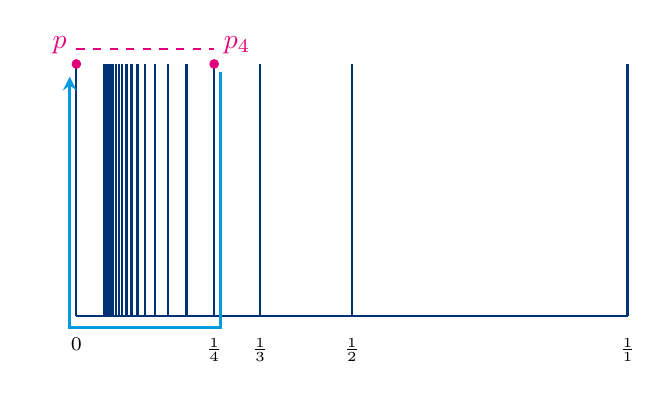
\begin{tikzpicture}[xscale=7, yscale=3.2]
  \draw[icnavy, thick] (0,0) -- (1,0);
  \draw[icnavy, thick] (0,0) -- (0,1);
  \foreach \n in {1,...,20} \draw[icnavy, thick] ({1/\n},0) -- ({1/\n},1);
  \draw[iccyan, very thick, ->, >=stealth] (0.262,0.97) -- (0.262,-0.045) -- (-0.012,-0.045) -- (-0.012,0.95);
  \draw[icmag, thick, dashed] (0,1.06) -- (0.25,1.06);
  \fill[icmag] (0,1) circle (0.25pt and 0.55pt) node[above left] {$p$};
  \fill[icmag] (0.25,1) circle (0.25pt and 0.55pt) node[above right] {$p_4$};
  \foreach \n in {1,2,3,4} \node[below] at ({1/\n},-0.05) {\scriptsize $\frac1{\n}$};
  \node[below] at (0,-0.05) {\scriptsize $0$};
\end{tikzpicture}
\caption{El peine. La distancia euclídea entre $p_n$ y $p$ es $1/n$ (en magenta), pero toda curva dentro del peine tiene que bajar y volver a subir (en cian), así que $d_L(p_n,p)\ge2$.}
\label{fig:peine}
\end{figure}

\begin{proposicion}\label{prop:misma-longitud}
Sea $\gamma\colon[a,b]\to X$ una curva.
\begin{enumerate}[label=(\alph*)]
\item Si $\gamma$ es continua para $d_L$, entonces es continua para $d$.
\item Si $\gamma$ es $d$-rectificable, entonces es continua para $d_L$.
\item Si $\gamma$ es continua para ambas métricas, entonces $L_{d_L}(\gamma)=L_d(\gamma)$ (como elementos de $[0,\infty]$).
\end{enumerate}
\end{proposicion}

\begin{proof}
(a) Es inmediato de $d\le d_L$.

(b) Para $s\le t$, la restricción $\gamma|_{[s,t]}$ une $\gamma(s)$ con $\gamma(t)$, así que, con $\ell$ la longitud acumulada respecto de $d$,
\[
d_L(\gamma(s),\gamma(t))\le L_d(\gamma|_{[s,t]})=\ell(t)-\ell(s).
\]
Como $\ell$ es continua (Lema~\ref{lem:continuidad}), $\gamma$ es continua para $d_L$.

(c) Como $d\le d_L$, cada suma sobre una partición calculada con $d$ es menor o igual que la calculada con $d_L$; tomando supremo, $L_d(\gamma)\le L_{d_L}(\gamma)$. Si $L_d(\gamma)=\infty$ no hay nada más que probar. Si $L_d(\gamma)<\infty$, para una partición $a=t_0<\dots<t_n=b$, cada tramo $\gamma|_{[t_{i-1},t_i]}$ une $\gamma(t_{i-1})$ con $\gamma(t_i)$, de modo que, por el Lema~\ref{lem:aditividad},
\[
\sum_{i=1}^n d_L(\gamma(t_{i-1}),\gamma(t_i)) \le \sum_{i=1}^n L_d\big(\gamma|_{[t_{i-1},t_i]}\big) = L_d(\gamma).
\]
Tomando supremo, $L_{d_L}(\gamma)\le L_d(\gamma)$.
\end{proof}

\begin{corolario}
$(d_L)_L=d_L$; es decir, $(X,d_L)$ es un espacio de longitud.
\end{corolario}

\begin{proof}
Por la Proposición~\ref{prop:misma-longitud}, las curvas $d_L$-rectificables son exactamente las curvas $d$-rectificables, y en ambas métricas tienen la misma longitud. Por lo tanto los ínfimos que definen $(d_L)_L$ y $d_L$ se toman sobre el mismo conjunto de números.
\end{proof}

Esto justifica llamar a $d_L$ la \emph{métrica intrínseca} inducida por $d$: aplicar la construcción una segunda vez ya no cambia nada. Además, $d=d_L$ si y sólo si $(X,d)$ es un espacio de longitud.

\section{Reparametrización por longitud de arco}

\begin{proposicion}\label{prop:reparam}
Sea $\gamma\colon[0,1]\to X$ una curva rectificable de longitud $L>0$ y sea $\ell(t):=L(\gamma|_{[0,t]})$. Existe una curva $\tilde\gamma\colon[0,1]\to X$, con los mismos extremos y la misma imagen que $\gamma$, tal que $\gamma=\tilde\gamma\circ(\ell/L)$ y
\[
d\big(\tilde\gamma(s),\tilde\gamma(t)\big)\le L|t-s|,\qquad L\big(\tilde\gamma|_{[s,t]}\big)=L(t-s)\qquad(0\le s\le t\le1).
\]
\end{proposicion}

\begin{proof}
Por el Lema~\ref{lem:continuidad}, $\ell/L\colon[0,1]\to[0,1]$ es continua, no decreciente y suryectiva. Dado $s\in[0,1]$, definimos $\tilde\gamma(s):=\gamma(t)$ para cualquier $t$ con $\ell(t)=sL$. Está bien definida: si $\ell(t)=\ell(t')$ con $t\le t'$, entonces $d(\gamma(t),\gamma(t'))\le L(\gamma|_{[t,t']})=\ell(t')-\ell(t)=0$. Por construcción $\gamma=\tilde\gamma\circ(\ell/L)$, y $\tilde\gamma$ tiene los mismos extremos y la misma imagen que $\gamma$.

Si $\ell(t)=sL$ y $\ell(t')=s'L$ con $s\le s'$ (y entonces podemos tomar $t\le t'$),
\[
d(\tilde\gamma(s),\tilde\gamma(s'))=d(\gamma(t),\gamma(t'))\le\ell(t')-\ell(t)=L(s'-s).
\]
En particular, $\tilde\gamma$ es continua. Para la longitud, las particiones de $[t,t']$ se transforman por $\ell/L$ en particiones de $[s,s']$ (eventualmente con puntos repetidos, que no aportan a la suma), y toda partición de $[s,s']$ proviene de este modo de una de $[t,t']$, porque $\ell/L$ es suryectiva y monótona. Como $\gamma=\tilde\gamma\circ(\ell/L)$, las sumas correspondientes coinciden, y entonces $L(\tilde\gamma|_{[s,s']})=L(\gamma|_{[t,t']})=\ell(t')-\ell(t)=L(s'-s)$.
\end{proof}

En particular, $\tilde\gamma$ tiene velocidad métrica constante $L$. En general esto \emph{no} implica que $d(\tilde\gamma(s),\tilde\gamma(t))=L|t-s|$: esa igualdad caracteriza a las geodésicas (Definición~\ref{def:geodesica}). Si $L=0$, la curva es constante y no hace falta reparametrizarla.

\section{Geodésicas y el teorema de Hopf--Rinow}

\begin{definicion}\label{def:geodesica}
Una \emph{geodésica} (minimizante, parametrizada a velocidad constante) entre $x$ e $y$ es una curva $\gamma\colon[0,1]\to X$ con $\gamma(0)=x$, $\gamma(1)=y$ y
\[
d\big(\gamma(s),\gamma(t)\big)=|t-s|\,d(x,y)\qquad(s,t\in[0,1]).
\]
El espacio $(X,d)$ es un \emph{espacio geodésico} si todo par de puntos está unido por una geodésica.
\end{definicion}

Toda geodésica entre $x$ e $y$ tiene longitud $d(x,y)$. Recíprocamente, si una curva rectificable $\gamma$ une $x$ con $y$ y $L(\gamma)=d(x,y)$, su reparametrización por longitud de arco es una geodésica. En particular, todo espacio geodésico es un espacio de longitud, en el que además el ínfimo de la definición se alcanza.

Por ejemplo, $(S^1,d_L)$ y $(S^2,d_L)$ son espacios geodésicos: las geodésicas son los arcos más cortos de círculo máximo, recorridos a velocidad constante. En cambio, con la distancia euclídea, $S^1$ y $S^2$ no tienen geodésicas entre puntos distintos (Ejemplo~\ref{ej:esfera}).

\begin{ejemplo}[Las geodésicas no tienen por qué ser únicas]\label{ej:l1}
En $\mathbb R^2$ con la distancia euclídea, la única geodésica entre dos puntos es el segmento que los une. Pero si consideramos la distancia
\[
d_1(x,y)=|x_1-y_1|+|x_2-y_2|,
\]
hay muchas más. Sean $x=(0,0)$ e $y=(1,1)$, de modo que $d_1(x,y)=2$. El segmento $\gamma(t)=(t,t)$ es una geodésica, pero también lo es el camino que primero va hacia la derecha y después sube,
\[
\gamma(t)=\begin{cases}(2t,0)&\text{si }0\le t\le\frac12,\\(1,2t-1)&\text{si }\frac12\le t\le1.\end{cases}
\]
En efecto, si $s\le\frac12\le t$, entonces $d_1(\gamma(s),\gamma(t))=(1-2s)+(2t-1)=2(t-s)$, y si $s$ y $t$ están del mismo lado de $\frac12$ la cuenta es directa. Con el mismo argumento, cualquier ``escalera'' en la que ambas coordenadas son monótonas, recorrida a velocidad constante, es una geodésica (Figura~\ref{fig:l1}). Esta falta de unicidad no es una patología: va a aparecer también en los espacios de Wasserstein.
\end{ejemplo}

\begin{figure}[htbp]
\centering
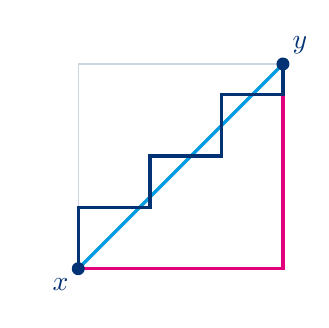
\begin{tikzpicture}[scale=2.6]
  \draw[icnavy!20] (0,0) rectangle (1,1);
  \draw[iccyan, very thick] (0,0) -- (1,1);
  \draw[icmag, very thick] (0,0) -- (1,0) -- (1,1);
  \draw[icnavy, very thick] (0,0) -- (0,0.3) -- (0.35,0.3) -- (0.35,0.55) -- (0.7,0.55) -- (0.7,0.85) -- (1,0.85) -- (1,1);
  \fill[icnavy] (0,0) circle (0.9pt) node[below left] {$x$};
  \fill[icnavy] (1,1) circle (0.9pt) node[above right] {$y$};
\end{tikzpicture}
\caption{Tres geodésicas distintas entre $x=(0,0)$ e $y=(1,1)$ para la distancia $d_1$: el segmento (cian), el camino en ``L'' (magenta) y una escalera (azul). Todas tienen longitud $d_1(x,y)=2$.}
\label{fig:l1}
\end{figure}

Un espacio métrico es \emph{propio} si sus bolas cerradas son compactas o, equivalentemente, si sus subconjuntos cerrados y acotados son compactos. Todo espacio propio es completo y localmente compacto.

\begin{teorema}[Hopf--Rinow para espacios métricos]\label{thm:HR}
Todo espacio de longitud propio es un espacio geodésico. Es decir, para todo $x,y\in X$ existe una geodésica $\gamma\colon[0,1]\to X$ entre $x$ e $y$; en particular, $L(\gamma)=d(x,y)$.
\end{teorema}

\begin{proof}
Pongamos $D=d(x,y)$. Si $D=0$, entonces $x=y$ y la curva constante sirve. Supongamos $D>0$.

Por ser $X$ un espacio de longitud, existen curvas $\gamma_n\colon[0,1]\to X$ que unen $x$ con $y$ y cumplen $D\le L(\gamma_n)\le D+1/n$. Como $L(\gamma_n)\ge D>0$, podemos reparametrizarlas por longitud de arco (Proposición~\ref{prop:reparam}); llamamos $\tilde\gamma_n$ a las curvas reparametrizadas, que tienen los mismos extremos y la misma longitud $L_n:=L(\gamma_n)$, y satisfacen
\[
d\big(\tilde\gamma_n(s),\tilde\gamma_n(t)\big)\le L_n|t-s|\le(D+1)|t-s|.
\]
Así, la familia $\{\tilde\gamma_n\}$ es equicontinua (de hecho, uniformemente Lipschitz). Además, para todo $t$,
\[
d(x,\tilde\gamma_n(t))\le L\big(\tilde\gamma_n|_{[0,t]}\big)\le L_n\le D+1,
\]
de modo que todas las imágenes están contenidas en la bola cerrada $\Bc(x,D+1)$, que es compacta por hipótesis.

Por el teorema de Arzelà--Ascoli (aplicado a funciones de $[0,1]$ en el compacto $\Bc(x,D+1)$), existe una subsucesión $\tilde\gamma_{n_k}$ que converge uniformemente a una curva continua $\gamma\colon[0,1]\to X$, con $\gamma(0)=x$ y $\gamma(1)=y$ (Figura~\ref{fig:HR}). Por el Lema~\ref{lem:sci},
\[
L(\gamma)\le\liminf_{k\to\infty}L(\tilde\gamma_{n_k})=\lim_{k\to\infty}L_{n_k}=D.
\]
Como siempre $D=d(x,y)\le L(\gamma)$, concluimos que $L(\gamma)=D$.

Para la última afirmación, pasando al límite en la desigualdad de Lipschitz se obtiene $d(\gamma(s),\gamma(t))\le D|t-s|$. Por otro lado, si $s\le t$, por la desigualdad triangular,
\[
D=d(x,y)\le d(x,\gamma(s))+d(\gamma(s),\gamma(t))+d(\gamma(t),y)\le Ds+d(\gamma(s),\gamma(t))+D(1-t),
\]
de donde $d(\gamma(s),\gamma(t))\ge D(t-s)$. Luego $d(\gamma(s),\gamma(t))=D|t-s|$.
\end{proof}

\begin{figure}[htbp]
\centering
\begin{tikzpicture}[scale=1.15]
  \draw[icnavy!40, dashed, thick] (0,0) circle (3.4);
  \node[icnavy!60, above left] at (135:3.4) {\small $\Bc(x,D+1)$};
  \foreach \A/\B/\c in {1.3/0.25/icnavy!25, -0.9/0.2/icnavy!40, 0.55/-0.12/icnavy!60, -0.3/0.08/icnavy!80}
    \draw[\c, thick] plot[domain=0:1, samples=100, smooth] ({2.4*\x}, {\A*sin(180*\x)+\B*sin(540*\x)});
  \draw[icmag, very thick] (0,0) -- (2.4,0);
  \fill[icnavy] (0,0) circle (1.4pt) node[left] {$x$};
  \fill[icnavy] (2.4,0) circle (1.4pt) node[right] {$y$};
  \node[icnavy!60] at (1.2,1.65) {\scriptsize $\tilde\gamma_{n_1}$};
  \node[icnavy!75] at (1.2,-1.2) {\scriptsize $\tilde\gamma_{n_2}$};
  \node[icmag] at (1.75,0.18) {\scriptsize $\gamma$};
\end{tikzpicture}
\caption{Idea de la demostración del Teorema~\ref{thm:HR}. Las curvas casi minimizantes $\tilde\gamma_{n_k}$ quedan dentro de la bola compacta $\Bc(x,D+1)$ y, por Arzelà--Ascoli, convergen a una curva $\gamma$ de longitud $d(x,y)$.}
\label{fig:HR}
\end{figure}

\begin{observacion}
El enunciado clásico de Hopf--Rinow--Cohn-Vossen pide que $X$ sea un espacio de longitud completo y localmente compacto, y prueba que entonces $X$ es propio; en ese contexto, el Teorema~\ref{thm:HR} es la parte que asegura la existencia de geodésicas. Acá tomamos directamente la propiedad como hipótesis, que es lo único que usa la demostración.
\end{observacion}

\subsection{Dos ejemplos sin compacidad local}\label{sec:ejemplos}

El Teorema~\ref{thm:HR} da una condición \emph{suficiente} para que un espacio sea geodésico. Los dos ejemplos que siguen muestran que, cuando falta la compacidad, puede pasar cualquier cosa: en ambos el espacio es completo, es de longitud y \emph{no} es localmente compacto, pero el primero es geodésico y el segundo no.

\begin{ejemplo}[Un espacio geodésico que no es localmente compacto]\label{ej:hilbert}
Sea $H$ un espacio de Hilbert de dimensión infinita (por ejemplo, $\ell^2$), con la distancia $d(x,y)=\|x-y\|$. Es completo por definición.

\emph{Es geodésico.} Dados $x,y\in H$, el segmento $\gamma(t)=(1-t)x+ty$ cumple
\[
\|\gamma(s)-\gamma(t)\|=\|(t-s)(x-y)\|=|t-s|\,\|x-y\|,
\]
así que es una geodésica entre $x$ e $y$ en el sentido de la Definición~\ref{def:geodesica}. En particular, $H$ también es un espacio de longitud.

\emph{No es localmente compacto.} Sea $\{u_k\}_{k\ge1}$ una sucesión ortonormal y sea $r>0$. Los puntos $x+r\,u_k$ están en la bola cerrada $\Bc(x,r)$, y para $k\ne j$,
\[
\|r\,u_k-r\,u_j\|=r\sqrt{\|u_k\|^2+\|u_j\|^2}=r\sqrt2.
\]
Como todos los puntos están a distancia $r\sqrt2$ entre sí, la sucesión no tiene ninguna subsucesión de Cauchy, y por lo tanto ninguna subsucesión convergente. Así, ninguna bola cerrada centrada en $x$ es compacta, por chica que sea.
\end{ejemplo}

\begin{ejemplo}[Un espacio de longitud completo que no es geodésico]\label{ej:grafo}
Tomamos dos puntos $x$ e $y$ y los unimos con infinitas aristas $e_1,e_2,e_3,\dots$, donde la arista $e_n$ es un segmento de longitud
\[
\ell_n:=1+\tfrac1n.
\]
Las aristas sólo se tocan en sus extremos $x$ e $y$ (Figura~\ref{fig:grafo}). Cada punto de $e_n$ queda determinado por su distancia $s\in[0,\ell_n]$ a $x$ medida \emph{a lo largo de la arista}. Llamamos \emph{camino} a una curva que se mueve por las aristas, y su longitud es la suma de los tramos recorridos en cada arista. Definimos
\[
d(p,q):=\inf\{\text{longitud de un camino de } p \text{ a } q\}.
\]
Llamemos $X$ al espacio resultante.

\begin{figure}[htbp]
\centering
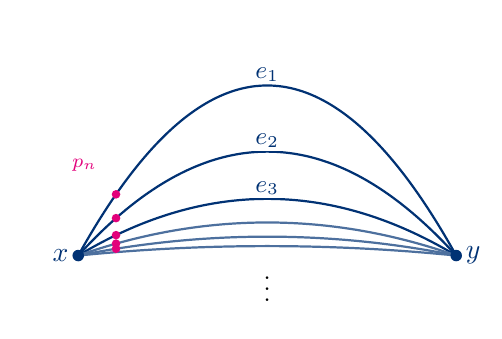
\begin{tikzpicture}[scale=1.6]
  \foreach \h/\lab in {1.8/e_1, 1.1/e_2, 0.6/e_3}{
    \draw[icnavy, thick] (0,0) .. controls (1,\h) and (2,\h) .. (3,0) node[pos=0.5,above,fill=white,inner sep=1pt] {\small $\lab$};
  }
  \foreach \h in {0.35, 0.2, 0.1}{
    \draw[icnavy!70, thick] (0,0) .. controls (1,\h) and (2,\h) .. (3,0);
  }
  \foreach \h in {1.8, 1.1, 0.6, 0.35, 0.2}{
    \path (0,0) .. controls (1,\h) and (2,\h) .. (3,0) node[pos=0.1, circle, fill=icmag, inner sep=1.1pt] {};
  }
  \node[icmag] at (0.05,0.72) {\scriptsize $p_n$};
  \fill[icnavy] (0,0) circle (1.3pt) node[left] {$x$};
  \fill[icnavy] (3,0) circle (1.3pt) node[right] {$y$};
  \node at (1.5,-0.2) {\small $\vdots$};
\end{tikzpicture}
\caption{El grafo del Ejemplo~\ref{ej:grafo}. Las aristas se van acortando: $e_n$ mide $1+\frac1n$. Los puntos $p_n$ (en magenta) están todos cerca de $x$, pero a distancia al menos $2r$ entre sí.}
\label{fig:grafo}
\end{figure}

La observación clave es la siguiente. Si sacamos los puntos $x$ e $y$, el espacio se parte en las aristas abiertas, que son disjuntas entre sí. Por lo tanto:

\begin{enumerate}[label=($\ast$)]
\item \emph{Una curva que sale de un punto interior de $e_n$ no puede entrar en otra arista sin pasar antes por $x$ o por $y$.}
\end{enumerate}

Esto se justifica por conexión: el tramo de la curva anterior a la primera visita a $\{x,y\}$ es un conjunto conexo que no contiene a $x$ ni a $y$, así que queda dentro de una única arista abierta. De ($\ast$) salen dos consecuencias:
\begin{enumerate}[label=(\roman*)]
\item Si $p\in e_n$ está a distancia $s$ de $x$ a lo largo de la arista, entonces $d(p,\{x,y\})=\min\{s,\ \ell_n-s\}$: para llegar a $x$ o a $y$ hay que recorrer la arista hasta uno de sus extremos.
\item Si $p$ y $q$ están en aristas distintas, entonces $d(p,q)\ge d(p,\{x,y\})+d(q,\{x,y\})$: todo camino de $p$ a $q$ tiene que llegar primero a $x$ o a $y$ y, al final, salir de $x$ o de $y$ hacia $q$.
\end{enumerate}

Veamos ahora las propiedades de $X$.

\emph{Es un espacio de longitud.} Si un camino recorre un tramo de arista de largo $s$, sus extremos están a distancia $d$ a lo sumo $s$. Por eso la longitud de un camino calculada con $d$ (como en la Sección~1) es menor o igual que la suma de los tramos recorridos. Tomando ínfimo sobre los caminos de $p$ a $q$, el ínfimo de las longitudes es a lo sumo $d(p,q)$; como siempre es al menos $d(p,q)$, coinciden.

\emph{Es completo.} Sea $(q_k)$ una sucesión de Cauchy. Hay dos casos.
\begin{itemize}
\item Si infinitos términos están en una misma arista $e_n$ (incluyendo sus extremos), esos términos forman una sucesión en $e_n$, que es compacta por ser imagen continua del intervalo $[0,\ell_n]$. Entonces tienen una subsucesión convergente.
\item Si no, podemos elegir una subsucesión $(q_{k_j})$ cuyos términos están en aristas distintas y no son $x$ ni $y$. Por (ii), $d(q_{k_j},q_{k_{j+1}})\ge d(q_{k_j},\{x,y\})$, y como la sucesión es de Cauchy, el lado izquierdo tiende a $0$. Luego $d(q_{k_j},\{x,y\})\to0$, y alguna subsucesión converge a $x$ o a $y$.
\end{itemize}
En ambos casos, $(q_k)$ es una sucesión de Cauchy con una subsucesión convergente, así que converge.

\emph{No es localmente compacto.} Fijemos $0<r\le\frac12$ y sea $p_n$ el punto de $e_n$ a distancia $r$ de $x$ a lo largo de la arista. Recorriendo la arista vemos que $d(x,p_n)\le r$, de modo que todos los $p_n$ están en la bola cerrada $\Bc(x,r)$. Por (i), $d(p_n,\{x,y\})=\min\{r,\ \ell_n-r\}=r$, ya que $\ell_n-r>1-r\ge r$. Por (ii), si $n\ne m$,
\[
d(p_n,p_m)\ge 2r.
\]
Como en el Ejemplo~\ref{ej:hilbert}, la sucesión $(p_n)$ no tiene subsucesiones convergentes, así que $\Bc(x,r)$ no es compacta. Esto vale para todo $r\le\frac12$, de modo que $x$ no tiene ningún entorno compacto.

\emph{No es geodésico.} Por un lado, recorriendo la arista $e_n$ se obtiene $d(x,y)\le\ell_n$ para todo $n$, así que $d(x,y)\le1$. Por otro lado, sea $\gamma$ cualquier curva de $x$ a $y$. Consideremos el último instante $t_0$ en que $\gamma$ pasa por $x$ antes de su primera visita a $y$, y el instante $t_1>t_0$ de esa primera visita a $y$. Entre $t_0$ y $t_1$ la curva no pasa ni por $x$ ni por $y$, así que, por ($\ast$), se queda dentro de una sola arista $e_n$, que recorre de punta a punta. Como para puntos cercanos de una misma arista la distancia $d$ coincide con la distancia medida a lo largo de la arista, tomando particiones finas se obtiene
\[
L(\gamma)\ge\ell_n=1+\tfrac1n>1.
\]
Esto muestra que $d(x,y)=1$ (el ínfimo de los $\ell_n$) y que \emph{ninguna} curva de $x$ a $y$ tiene longitud $d(x,y)$. Por lo tanto, $X$ no es geodésico.
\end{ejemplo}

\begin{observacion}[¿Dónde falla la demostración de Hopf--Rinow?]
En el Ejemplo~\ref{ej:grafo}, las curvas $\gamma_n$ que recorren $e_n$ forman una sucesión minimizante: $L(\gamma_n)=1+\frac1n\to d(x,y)$. Reparametrizadas por longitud de arco, son uniformemente Lipschitz, igual que en la demostración del Teorema~\ref{thm:HR}. Lo que falla es el paso de Arzelà--Ascoli: los puntos medios $\tilde\gamma_n(\frac12)$ están en aristas distintas y lejos de $x$ y de $y$, así que, por (ii), están a distancia mayor que $1$ entre sí, y no tienen subsucesiones convergentes. La sucesión minimizante existe, pero ``se escapa'' por infinitas direcciones distintas y no tiene límite (Figura~\ref{fig:escape}).

\begin{figure}[htbp]
\centering
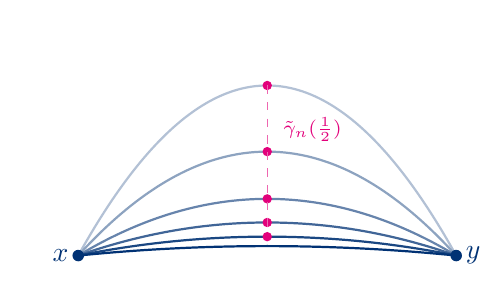
\begin{tikzpicture}[scale=1.6]
  \foreach \h/\c in {1.8/icnavy!30, 1.1/icnavy!45, 0.6/icnavy!60, 0.35/icnavy!75, 0.2/icnavy!90}{
    \draw[\c, thick] (0,0) .. controls (1,\h) and (2,\h) .. (3,0) node[pos=0.5, circle, fill=icmag, inner sep=1.2pt] {};
  }
  \draw[icnavy, thick] (0,0) .. controls (1,0.1) and (2,0.1) .. (3,0);
  \draw[icmag!60, dashed] (1.5,1.35) -- (1.5,0.2);
  \node[icmag, right] at (1.55,1.0) {\scriptsize $\tilde\gamma_n(\tfrac12)$};
  \fill[icnavy] (0,0) circle (1.3pt) node[left] {$x$};
  \fill[icnavy] (3,0) circle (1.3pt) node[right] {$y$};
\end{tikzpicture}
\caption{Los puntos medios $\tilde\gamma_n(\frac12)$ de las curvas minimizantes. Parecen acercarse a algo, pero están a distancia mayor que $1$ entre sí: no hay ningún punto límite, porque la ``arista de longitud $1$'' no existe.}
\label{fig:escape}
\end{figure}

La diferencia con el Ejemplo~\ref{ej:hilbert} no es que allí haya más compacidad en la topología de la métrica: en ninguno de los dos casos la hay. En el espacio de Hilbert las geodésicas existen por una razón distinta (allí se pueden escribir explícitamente). Más en general, para encontrar geodésicas en espacios que no son localmente compactos, una estrategia habitual es extraer límites de sucesiones minimizantes usando compacidad en una topología \emph{más débil} que la de la métrica, para la cual la longitud (o el costo que se quiera minimizar) siga siendo semicontinua inferiormente. Esta idea va a reaparecer en los espacios de Wasserstein.
\end{observacion}

\end{document}
